	\chapter{Implementierung}
	\label{chap:implementierung}
	
	\section{serielle Ausführung}
	\label{sec:seriellimplementierung}
	
	Der Code, mit dem die Ergebnisse dieser Arbeit berechnet wurden, befindet sich im Github-repository https://github.com/christianegross/bachelorarbeit. %Noch erneuern, wenn public
	
	Bei der Implementierung des Ising-Modells auf einem Rechner müssen noch weitere Randbedingungen vorgegeben werden:
	Das Gitter ist nicht unendlich lang, sondern begrenzt. Je größer das Gitter ist, desto näher ist das Ergebnis am thermodynamischen Limes. 
	Aufgrund der Begrenzung des Gitters müssen Annahmen für die Nachbarn der Teilchen am Rand des Gitters gemacht werden. Hier wurden periodische Randbedingungen gewählt, der Nachbar eines letzten Teilchen einer Zeile ist also das erste Teilchen der Spalte.
	
	Um die Auswertung der Messungen zu vereinfachen, wurden in dieser Arbeit $H$, $k_B$ und $T$ einheitenlos gewählt, und $k_B=1$ angenommen. Zudem wurde $J=1$ gesetzt.
	
	%Bei der Umsetzung ist nur ein endliches Gitter vorhanden.
	%Randbedingungen: Auch für die Spins am Rande des Gitters muss es Nachbarn geben. Hier wurden periodische Randbedingungen gewählt, d.h. der Nachbar von einem Punkt am Ende einer Zeile ist der Punkt am Anfang der Zeile.
	%Um Messungen zu vereinfachen: setze $k_B=1$, betrachte nur $T$.
	Bei einer Messung wird bei jedem Spin im Gitter ein Metropolis-Update durchgeführt.%Eine Messung: Bei jedem Spin wird ein Metropolis-Update durchgeführt.
	Dabei werden verschiedene Dinge gemessen: \begin{itemize}
		\item Der Hamiltonian des Systems, dies nach Gl.\ref{eq:hamiltonianising}
		\item Die Akzeptanzrate des Systems, also bei welchem Anteil der Spins das Metropolis-Update zur Umdrehung geführt hat. Dies wird für jedes einzelne Update gezählt und am Ende gemittelt.
		\item Die Magnetisierung des Systems nach Gl.~\ref{eq:magnetisierung}. 
		%\item Das Quadrat und die vierte Potenz der Magnetisierung, um die Cumulante bestimmen zu können
	\end{itemize}
	%Akzeptanzrate: Wie viele Spins wurden bei einer Messung umgedreht? Wird bei jedem Punkt gezählt und in eine Variable geschrieben.
	
	%Magnetisierung: Betrag der Summe über alle Spins im Gitter, je mehr Spins gleich ausgerichtet sind, desto stärker der nach außen sichtbare Effekt als Magnet. Nach jeder Messung bestimmt.
	Aufgrund der endlichen Gitterlänge kann es vorkommen, dass das Vorzeichen der Magnetisierung während der Beobachtung wechselt. Um dadurch keine unstetigen Messungen zu erhalten, wird der Betrag der Magnetisierung gemessen~\cite[vgl. ][S. 106 ff.]{binderheermann}.%Um diesen Effekt nicht fälschlicherweise zu berücksichtigen, wird der Betrag der Magnetisierung gemessen~\cite[vgl. ][S. 106 ff.]{binderheermann}.
	
	
	Das Gitter wird als eindimensionales \textit{Array} abgespeichert. Das Element an Position (x,y) ist dann der $\text{laenge}\cdot\text{x}+\text{y}$-te Eintrag des \textit{Arrays} (alles in C-Zählweise, also bei 0 angefangen).

	Der Hamiltonian des Gitters wird in der Funktioen \texttt{hamiltonian} berechnet, indem das Gitter zeilenweise durchgegangen wird und von jedem Teilchen die Interaktionsenergie mit dem rechten und dem unteren Nachbarn zum bisherigen Hamiltonian addiert wird.
	
	Die zur Durchführung des Metropolis-Update benötigte Energiedifferenz bei Umdrehung eines Spin wird berechnet, indem die Energiedifferenz zu den nächsten vier Nachbarn berechnet wird. Dies geschieht in der Funktione\texttt{deltahneu2}.
	Nach~\cite[S. 103]{binderheermann} kann diese Energiedifferenz nur einer von fünf Werten sein. Daher wird die Wahrscheinlichkeit für die Spindrehung nicht jedes mal neu berechnet, sondern in einem \textit{Array} nachgeschaut.
	
	Um zu erreichen, dass der \textit{Spinflip} mit der entsprechenden Wahrscheinlichkeit angenommen wird, wird die Wahrscheinlichkeit mit einer Zufallszahl zwischen null und eins verglichen\cite[nach][]{metropolisupdate}. Wenn die Wahrscheinlichkeit größer als die Zufallszahl ist, wird der \textit{Spinflip} ausgeführt, und die Energiedifferenz zum Hamiltonian dazu addiert. 
	
	Die Messung wird in der Funktion \texttt{sweepaltohnepar} durchgeführt, in der in \texttt{for}-Schleifen das ganze Gitter durchgegangen wird. Für jeden Punkt wird die Energiedifferenz bei Umdrehung ermittelt und damit ein Metropolis-Update durchgeführt. Falls der Spin umgedreht wird, werden Hamiltonian und Akzeptanzrate aktualisiert. Nachdem bei jedem Punkt ein Update durchgeführt worden ist, wird die Magnetisierung als summe über alle Gitterelemente berechnet und die gemessenen Observablen werden in eine \texttt{.txt}-Datei ausgegeben, in der die Ergebnisse aller Messungen gespeichert werden.
	%Hamiltonian: berechnen über zeilenweise \textit{Array} durchgehen, von jedem Punkt rechten und unteren Nachbarn, periodische Randbedingungen durch modulo.
	%Metropolis-Update: Nur vier Nachbarn zum Berechnen nötig, Hamiltonian wird als Parameter übergeben, daraus Änderung bei Flip, Akzeptanz wird durch 0/1 zurückgegeben. Wahrscheinlichkeit für Flip: Vergleich mit Zufallszahl zwischen null und eins.
	%sweep Funktion: geht das ganze Gitter durch und führt bei jedem Punkt ein Metropolis-Update durch. Zählt wie viele Spins geflippt werden, schreibt am Ende Prozentuale Veränderungen (Akzeptanzrate) und Summe über alle Spins(Magnetisierung) in Ausgabedatei.
	
	%Um eine zufällige Anfangskonfiguration zu erzeugen, wird ein eindimensionales \textit{Array} mit laenge$\cdot$laenge Einträgen erstellt. Mithilfe von Zufallszahlen wird jedem Element des \textit{Arrays} zufällig $1$ oder $-1$ zugeteilt.	
	%Initialisierung des Gitters: Als 1D \textit{Array} abspeichern, mit Mersenne Twister $\pm1$ auf das Gitter verteilen.
	
	Die Anfangskonfiguration wird in der Funktion \texttt{initialisierung} erzeugt. Dort gibt es die Möglichkeit, mittels mit dem \texttt{gsl\_rng}-Paket\cite{gsldoc} erzeugter Zufallszahlen $\pm 1$ auf das Gitter zu verteilen, im Verlauf der Messungen hat es sich allerdings herausgestellt, das es sinnvoll ist, mit einem Gitter anzufangen, bei dem alle Elemente gleich sind. 
	
	%, deren Ergebnisse nicht verwendet werden. 
	Um das Gitter zu thermalisieren, werden Messungen an Zuständen durchgeführt, die sich nicht im Gleichgewicht befinden und daher nicht in das Ergebnis mit einfließen. Wie viele solcher Messungen hängt von der Temperatur ab, da sich bei einigen Temperaturen die Observablen sehr schnell ändern und bei anderen weniger schnell. Als Basis für die erste betrachtete Temperatur wird ein vollkommen homogenes Gitter, an dem $\num{1000}$ Messungen durchgeführt wurden, angenommen. Für alle anderen Gitter wird das thermalisierte Gitter der davor behandelten Temperatur als Basis angenommen. An allen Basisgittern werden weitere Messungen zur Thermalisierung vorgenommen: Nach ersten Messungen liegt ein kritischer Punkt zwischen $T=\num{2,25}$ und $T=\num{2,4}$, deshalb werden bei allen Gittern, die bei diesen Temperaturen betrachtet werden, $\num{20000}$ Thermalisierungsschritte durchgeführt. Für alle anderen Gitter zwischen $T=\num{2}$ und $T=\num{3}$ werden $\num{10000}$, für alle Gitter außerhalb dieser Temperaturen $\num{5000}$ Schritte durchgeführt.
	%Ein kritischer Punkt scheint zwischen $T=\num{2,25}$ und $T=\num{2,4}$ zu liegen
	%Messungen zeigen: dauert vor allem bei kleinen Gittern sehr lange, bis bei kleiner Temperatur Gleichgewicht erreicht ist. Daher: Am Anfang komplett geordnet, alles $-1$. 
	%Recht nah an Gleichgewichtszustand, daher für ersten Zustand 1000 Thermalisierungen vor Beginn der Schleife. In Schleife: Anzahl an Thermalisierungen abhängig von Temperatur, Messungen ergeben kritischen Bereich mit vielen Veränderungen zwischen $T=\num{2,25}$ und $T=\num{2,4}$, daher in diesem Bereich 100.000, zwischen $T=\num{2}$ und $T=\num{3}$ 30.000, sonst 5.000. Thermalisierung aufgrund des Gitters der Temperatur, die davor behandelt wurde.
	%Diese zufällige Konfiguration ist weit vom interessanten Gleichgewicht entfernt, sodass die ersten Messungen nicht verwendet werden können. Daher ist am Anfang eine Thermalisierung nötig, nach der sich das System im Gleichgewicht befindet. Für die erste Temperatur werden (10.000) Messungen durchgeführt und verworfen, für alle Temperaturen danach wird das Gitter der vorherigen Temperatur übergeben und mit (5.000) Messungen thermalisiert. 
	Das thermalisierte Gitter wird ausgegeben und kann somit auch für spätere Messungen wieder verwendet werden. Die Datei mit den Messergebnissen der Thermalisierung ist nicht relevant und wird daher von weiteren Thermalisierungsmessungen überschrieben.
	
	Beim Messen wird die gewünschte Anzahl an Messungen als Parameter übergeben, die Messungen werden in eine Datei geschrieben. Als Basis für die Messungen wird das zuvor thermalisierte Gitter angenommen.
	
	Aus den Messdaten werden, wie in Abschnitt~\ref{sec:theorieauswertung} erläutert, sowohl die naiven Standardschätzer nach Gl.~\ref{eq:standardmitteundfehler} als auch Schätzer mit \textit{Blocking} und \textit{Bootstrapping} für Mittelwert und Standardabweichung der Magnetisierung, der Akzeptanzrate und des Hamiltonian bestimmt.
	
	Dazu werden die Daten wieder eingelesen. Das \textit{Bootstrapping} wird mit verschiedenen Blocklängen durchgeführt, für jede Blocklänge wird allerdings die gleiche Anzahl, nämlich $4\cdot\text{Anzahl der Messungen}$, \textit{Replicas} gezogen
	
	%Am Anfang Einbrennen nötig: Gitter der vorherigen Temperatur wird übergeben, N0 (=10.000) Messungen werden durchgeführt, deren Ergebnisse nicht verwendet werden, da sie zu stark variieren, Gitter nach Einbrennen wird in .txt Datei gespeichert.
	
	%Danach messen: Ergebnisse werden in Ausgabedatei geschrieben.
	
	%Die Daten der Messdatei werden wieder eingelesen, um daraus den naiven Mittelwert $\mu=\frac{1}{N}\sum_{i} x_i$ und die naive Standardabweichung $\sigma=\frac{1}{N-1}\sum_{i}(x_i-\mu)^2$ zu bilden. Diese werden zusammen mit Temperatur und Gitterlänge in eine Datei geschrieben.
	%Aus Datei durch einlesen mit Standardschätzern naiven Mittelwert $\mu=\frac{1}{N}\sum_{i} x_i$ bilden und damit Standardabweichung $\sigma=\frac{1}{N-1}\sum_{i}(x_i-\mu)^2$ berechnen. Temperatur, Mittelwert und Varianz der Akzeptanzrate und Magnetisierung werden in Datei geschrieben.
	
	%Da es sich um Markov-Chain-Monte-Carlo handelt, sind die Konfigurationen nicht voneinander unabhängig, also autokorreliert. Insbesondere ist diese Autokorrelation temperaturabhängig(warum? Zitat).
	
	%Um die Autokorrelation zu verringern, werden die Mittelwerte und Fehler der Messdaten zusätzlich noch durch Bootstrapping mit vorherigem Blocking bestimmt. Das Blocking sorgt dafür, dass die Autokorrelation kleiner wird, dass Bootstrapping dafür, dass die ermittelten Werte eher der zugrundeliegenden Wahrscheinlichkeitsverteilung entsprechen. Die Werte zur Erzeugung der Blöcke werden wiederum aus der \texttt{.txt}-Datei mit den Messergebnissen eingelesen.
	
%	Fehler kommen durch Autokorrelation der Daten, sind also Temperaturabhängig: Beseitigung der Autokorrelation durch Blocking der Daten, also Einteilen in verschiedene Blöcke der Länge $l$, danach Bootstrapping, um Fehlerqualität zu verbessern. (Zitat?)
	%Bootstrapping: zur Erzeugung eines Replikas aus Messwerten so viele Werte mit Zurücklegen ziehen, wie es Messungen gibt und daraus den arithmetischen Mittelwert bilden. Aus $r$ so gebildeten Replikas den Standardschätzer für Mittelwert und Varianz ziehen. Temperatur, $l$, Mittelwert und Varianz in Datei schreiben.
	
	%\cite{skriptcompphys}
	
	%Der so berechnete Fehler hängt von der Länge l der Blöcke ab, er steigt mit der Länge. Ab einer gewissen Länge bleiben die Fehler konstant, diese Region eignet sich gut, um temperaturunabhängige Fehler zu bestimmen.
	%So errechneter Fehler steigt mit l an, ab einer gewissen Länge bildet sich ein Plateau. Quelle: Skript.
	
	%Bild Fehler in Abhängigkeit von l? %Erklärung Bootstrapping? Zitate?
	
	Zur Bestimmung des kritischen Punktes wird ausgenutzt, dass an diesem eine Unstetigkeit in der Magnetisierung besteht. Aufgrund der endlichen Länge des Gitters gibt es keine Unstetigkeit in der Ableitung der Magnetisierung, sondern nur ein Extremum. Dieses wird bestimmt, indem das Minimum der mit der 2-Punkt-Formel gebildeten Ableitung bestimmt wird. Der Fehler der Ableitung wird mittels Gaußscher Fehlerfortpflanzung bestimmt.
	%Kritischer Punkt: Unstetigkeit in Magnetisierung/Pol in Ableitung erwartet, bestimmen über größte Änderung/Extremum der Ableitung der Magnetisierung: Mit 2-Punkt-Formel berechnete Ableitung, Fehler der Ableitung mit Gaußscher Fehlerfortpflanzung ermittelt.
		
	Die Magnetisierung bei vielen Temperaturen wird im Programm \texttt{ising.c} gemessen. Dazu werden in der \texttt{main}-Funktion Variablen wie $J$, der Zufallszahlengenerator und ein \textit{Array} für die Temperaturen initialisiert. Außerdem wird die Gitterlänge, die Anzahl an Messungen und Thermalisierungsschritten vor der ersten Temperatur sowie die Länge der Blöcke fürs \textit{Bootstrapping} festgelegt. 	
	%Main-funktion: Variablen wie T, J, N0 initialisieren, \textit{Array} mit verwendeten Temperaturen und l fürs Bootstrapping erzeugen, Dateien für Mittelwerte öffnen
	
	Zuerst wird ein Gitter erstellt, initialisiert und zum ersten Mal bei der niedrigsten betrachteten Temperatur thermalisiert. Danach werden in einer for-Schleife alle gewählten Temperaturen aufsteigend bearbeitet, bei jeder Temperatur wird das Gitter erst thermalisiert und danach die gewünschte Zahl an Messungen durchgeführt.
	%Messungen für verschiedene Temperaturen: Durch for-Schleife, vorher Initialisierung eines Array, in das die Temperaturen gleichmäßig verteilt hineingeschrieben werden.
	Die Messergebnisse werden in einer \texttt{.txt}-Datei gespeichert. Danach wird aus den Messwerten sowohl mit der naiven Methode, als auch mit \textit{Blocking} und \textit{Bootstrapping}, der Mittelwert sowie die Standardabweichung der Magnetisierung, der Akzeptanzrate und des Hamiltonians bei der gegebenen Temperatur bestimmt.
	%Initialisierung mit (100.000) Messungen am ersten Gitter, danach Thermalisierung mit Gitter der vorherigen Temperatur.
	%for-Schleife über alle Temperaturen im array: Datei für Gitter, Messergebnisse öffnen, thermalisieren, messen, naive Schätzer und Bootstrapschätzer für verschiedene l bestimmen.
	
	Die Ableitung sowie deren Minimum werden mit dem Programm \texttt{minline.c} bestimmt. Hierbei werden für verschiedene Gitterlängen jeweils die Bootstrapergebnisse der Magnetisierung eingelesen, deren Ableitung bestimmt sowie die Zeile, in der die Ableitung ein Minimum hat, auf die Standardausgabe geschrieben.
	%Am Ende des Programms wird aus den ermittelten Werten die Ableitung der Magnetisierung berechnet und ebenfalls in eine \texttt{.txt}-Datei geschrieben.
	%Am Ende Ableitung in separate Datei schreiben.
		
	
	\section{parallele Ausführung}
	\label{sec:parallelimplementierung}


	
	Die zum Messen benötigte Zeit steigt mit dem Quadrat der Gitterlänge. Dies sorgt vor allem bei den interessanten langen Gitterlängen, die näher an den thermodynamischen Limes herankommen, für lange Messzeiten. Um diese Messungen zu beschleunigen, wurde das Programm parallelisiert.
	
	\subsection{Parallelisierung mit OpenMP}
	\label{subsec:paropenmp}
	Bei der Parallelisierung mit OpenMP wurden rechenintensive \texttt{for}-Schleifen parallelisiert.
	%Einzelne Messung dauert recht lange: Beschleunigen durch parallelisieren. 
	%Strategie: Vor allem Rechenintensive Bereiche parallelisieren, z.B. sweep-funktion für Messvorgang und Replikas ziehen.
	%Parallelisiert: \texttt{for}-Schleifen, deren Ausführungen unabhängig vom vorherigen Schleifendurchgang sind.
	
%	
%	\begin{wrapfigure}{r}{3.5in}
%		%\begin{figure}[htbp]
%		\centering
%		% GNUPLOT: LaTeX picture with Postscript
\begingroup
  \makeatletter
  \providecommand\color[2][]{%
    \GenericError{(gnuplot) \space\space\space\@spaces}{%
      Package color not loaded in conjunction with
      terminal option `colourtext'%
    }{See the gnuplot documentation for explanation.%
    }{Either use 'blacktext' in gnuplot or load the package
      color.sty in LaTeX.}%
    \renewcommand\color[2][]{}%
  }%
  \providecommand\includegraphics[2][]{%
    \GenericError{(gnuplot) \space\space\space\@spaces}{%
      Package graphicx or graphics not loaded%
    }{See the gnuplot documentation for explanation.%
    }{The gnuplot epslatex terminal needs graphicx.sty or graphics.sty.}%
    \renewcommand\includegraphics[2][]{}%
  }%
  \providecommand\rotatebox[2]{#2}%
  \@ifundefined{ifGPcolor}{%
    \newif\ifGPcolor
    \GPcolortrue
  }{}%
  \@ifundefined{ifGPblacktext}{%
    \newif\ifGPblacktext
    \GPblacktextfalse
  }{}%
  % define a \g@addto@macro without @ in the name:
  \let\gplgaddtomacro\g@addto@macro
  % define empty templates for all commands taking text:
  \gdef\gplbacktext{}%
  \gdef\gplfronttext{}%
  \makeatother
  \ifGPblacktext
    % no textcolor at all
    \def\colorrgb#1{}%
    \def\colorgray#1{}%
  \else
    % gray or color?
    \ifGPcolor
      \def\colorrgb#1{\color[rgb]{#1}}%
      \def\colorgray#1{\color[gray]{#1}}%
      \expandafter\def\csname LTw\endcsname{\color{white}}%
      \expandafter\def\csname LTb\endcsname{\color{black}}%
      \expandafter\def\csname LTa\endcsname{\color{black}}%
      \expandafter\def\csname LT0\endcsname{\color[rgb]{1,0,0}}%
      \expandafter\def\csname LT1\endcsname{\color[rgb]{0,1,0}}%
      \expandafter\def\csname LT2\endcsname{\color[rgb]{0,0,1}}%
      \expandafter\def\csname LT3\endcsname{\color[rgb]{1,0,1}}%
      \expandafter\def\csname LT4\endcsname{\color[rgb]{0,1,1}}%
      \expandafter\def\csname LT5\endcsname{\color[rgb]{1,1,0}}%
      \expandafter\def\csname LT6\endcsname{\color[rgb]{0,0,0}}%
      \expandafter\def\csname LT7\endcsname{\color[rgb]{1,0.3,0}}%
      \expandafter\def\csname LT8\endcsname{\color[rgb]{0.5,0.5,0.5}}%
    \else
      % gray
      \def\colorrgb#1{\color{black}}%
      \def\colorgray#1{\color[gray]{#1}}%
      \expandafter\def\csname LTw\endcsname{\color{white}}%
      \expandafter\def\csname LTb\endcsname{\color{black}}%
      \expandafter\def\csname LTa\endcsname{\color{black}}%
      \expandafter\def\csname LT0\endcsname{\color{black}}%
      \expandafter\def\csname LT1\endcsname{\color{black}}%
      \expandafter\def\csname LT2\endcsname{\color{black}}%
      \expandafter\def\csname LT3\endcsname{\color{black}}%
      \expandafter\def\csname LT4\endcsname{\color{black}}%
      \expandafter\def\csname LT5\endcsname{\color{black}}%
      \expandafter\def\csname LT6\endcsname{\color{black}}%
      \expandafter\def\csname LT7\endcsname{\color{black}}%
      \expandafter\def\csname LT8\endcsname{\color{black}}%
    \fi
  \fi
    \setlength{\unitlength}{0.0500bp}%
    \ifx\gptboxheight\undefined%
      \newlength{\gptboxheight}%
      \newlength{\gptboxwidth}%
      \newsavebox{\gptboxtext}%
    \fi%
    \setlength{\fboxrule}{0.5pt}%
    \setlength{\fboxsep}{1pt}%
\begin{picture}(5040.00,5040.00)%
    \gplgaddtomacro\gplbacktext{%
      \csname LTb\endcsname%
      \put(2356,4401){\makebox(0,0){\strut{}}}%
    }%
    \gplgaddtomacro\gplfronttext{%
      \csname LTb\endcsname%
      \put(630,103){\makebox(0,0){\strut{}$0$}}%
      \put(1397,103){\makebox(0,0){\strut{}$2$}}%
      \put(2165,103){\makebox(0,0){\strut{}$4$}}%
      \put(2931,103){\makebox(0,0){\strut{}$6$}}%
      \put(3699,103){\makebox(0,0){\strut{}$8$}}%
      \put(250,3888){\makebox(0,0)[r]{\strut{}$0$}}%
      \put(250,3157){\makebox(0,0)[r]{\strut{}$2$}}%
      \put(250,2426){\makebox(0,0)[r]{\strut{}$4$}}%
      \put(250,1696){\makebox(0,0)[r]{\strut{}$6$}}%
      \put(250,965){\makebox(0,0)[r]{\strut{}$8$}}%
    }%
    \gplbacktext
    \put(0,0){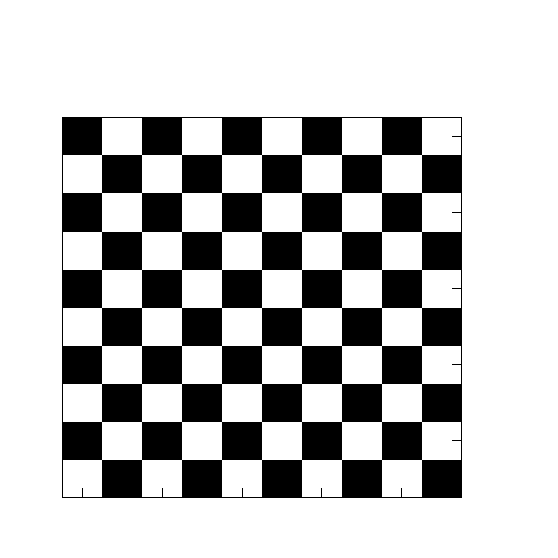
\includegraphics{schachbrett}}%
    \gplfronttext
  \end{picture}%
\endgroup

%		\caption{Schachbrettmuster}
%		\label{fig:schachbrett}
%		%\end{figure}
%	\end{wrapfigure}
%	
	Insbesondere bei der \texttt{sweep}-Funktion, die bei jedem Spin ein Metropolis-Update durchführt, lohnt sich eine Parallelisierung. Hierfür müssen jedoch die einzelnen Schleifendurchführungen unabhängig voneinander sein. Dies ist beim einfachen zeilenweise Durchgehen nicht der Fall. 
	Um die einzelnen Schleifendurchläufe unabhängig voneinander zu machen, wird das Gitter in zwei Untergitter aufgeteilt, die nacheinander abgearbeitet werden. Dies ist möglich, da für ein Update nur benötigt wird, dass die vier direkten Nachbarn unverändert sind. Daher lässt sich das Gitter in \enquote{schwarze}
	und \enquote{weiße} Punkte aufteilen, ähnlich einem Schachbrettmuster. % wie in Abb.~\ref{fig:schachbrett}. 
	Um ein Update an einem \enquote{schwarzen} Punkt durchzuführen, werden nur \enquote{weiße} Punkte benötigt und umgekehrt. Die \enquote{schwarzen} Punkte sind dadurch definiert, dass die Summe der Koordinaten eine gerade Zahl ist, die Summe der Koordinaten der \enquote{weißen} Punkte ist ungerade. Diese Aufteilung ist nur für gerade Gitterlängen möglich.
	
	Die Parallelisierung von \texttt{for}-Schleifen ist eine Standardanwendung von OpenMP und wird durch \textit{Compiler-Pragmas} eingebaut. In jedem Schleifendurchlauf wird die Akzeptanzrate sowie die Änderung des Hamiltonians gemessen. Bei der Parallelisierung ist es wichtig, dass nicht mehrere \textit{Threads} gleichzeitig versuchen, eine Variable zu verändern. Deshalb werden die entsprechenden Variablen zur Messung von Hamiltonian und Akzeptanzrate als privat deklariert, sodass jeder \textit{Thread} eine eigene Kopie der Variable bekommt. Erst am Ende der Messung werden ein einer kritischen Region, die nur ein \textit{Thread} zu einer Zeit durchführen kann, die Änderungen zusammengeführt. 	%sweep: bei zeilenweise durchgehen des Gitters von vorheriger Änderung abhängig.
	%Unabhängig: Gitter wie Schachbrett sehen, Update der Schwarzen Felder hängt nur von weißen ab und umgekehrt. Aufspalten in zwei separate \texttt{for}-Schleifen, eine Farbe pos1+pos2 gerade, andere ungerade. Einzelne Schleifen parallelisieren, Updates von Hamiltonian/Anzahl der geänderten Variablen in eigene Zwischenvariablen, Updaten in einer critical region(nur ein Thread kann Region zu einer Zeit ausführen) am Ende der Schleife.
	
	%Replikas ziehen: Gezogene Replikas werden in array geschrieben: Vollkommen unabhängig, parallelisieren der for-Schleife.
	
	Zusätzlich ist es wichtig, dass jeder \textit{Thread} auf einen eigenen Zufallszahlengenerator zugreift. Dies lässt sich nicht durch die Deklarierung des Generators als privat erreichen, sondern wird dadurch erreicht, dass nicht ein einzelner Generator, sondern ein \textit{Array} von Generatoren als Parameter an die \texttt{sweep}-Funktion übergeben wird.
	
	In der seriellen Ausführung der \texttt{sweep}-Funktion gibt es zwei ineinander geschachtelte \texttt{for}-Schleifen, die dafür sorgen, dass das gesamte Gitter einmal zeilenweise durchgegangen wird.
	
	In der parallelen Funktion \texttt{sweepmehreregeneratoren} wurde dies durch zwei Schleifenpaare ersetzt, eins für die \enquote{schwarzen} Punkte und eins für die \enquote{weißen} Punkte.
	Dafür wurden die Schleifenköpfe des seriellen Durchgangs so modifiziert, dass in jeder Zeile nur bei jedem zweiten Punkt ein Metropolis-Update durchgeführt wird. 
	\begin{verbatim}
	for (d1=0; d1<laenge;d1+=1){
		for (d2=(d1%2); d2<laenge; d2+=2){
	\end{verbatim}
	Hierbei sind \texttt{d1} und \texttt{d2} die Koordinaten und \texttt{laenge} die Länge des Gitters. Dadurch, dass die zweite Schleife mithilfe eines Modulo-Operators initialisiert wird, springt für jede Zeile die Position der betrachteten Punkte, wie es für ein Schachbrettmuster nötig ist. Um die weißen Punkte zu betrachten, wurde \texttt{(d1\%2)} durch \texttt{((d1+1)\%2)} ersetzt.
	% Auch in diesen Schleifen wird das ganze Gitter abgegangen, um Schleifendurchläufe zu verhindern, bei denen die Punkte der falschen Farbe untersucht werden, wird in der inneren Schleife nur jeder zweite Punkt berücksichtigt.
	%Statt einer Schleife zwei, andere Initialisierung für schwarz/weiß
	
	%Jede Parallelisierung führt zu mehr \textit{Overhead}, also zusätzlich benötigten Rechnungen. Falls es viel \textit{Overhead} gibt, wird zu dessen Ausführung genauso viel oder sogar mehr Zeit gebraucht, wie durch die Parallelisierung eingespart wurde.
	
	Da bei einem großen Anteil an \textit{Overhead} im Vergleich zu den eigentlichen Rechnungen eine Parallelisierung keinen Vorteil bietet, werden einige Funktionen, die zwar gut parallelisierbar wären, aber nicht lange zur Ausführung benötigen, wie z.B die Berechnung des Hamiltonians oder die Berechnung der Summe über alle Gitterelemente, nicht parallelisiert. Im Programm \texttt{ising.c} werden die Funktionen \texttt{thermalisieren, messen} und \texttt{sweepaltohnpar} durch \texttt{thermalisierenmehreregeneratoren, messenmehreregeneratoren} und \texttt{sweepmehreregeneratoren} ersetzt.
	
	Die benötigte Rechenzeit in Abhängigkeit der verwendeten Kerne wird im Programm \texttt{skalierung.c} gemessen. In diesem Programm werden erst Parameter wie Gitterlänge, untersuchte Temperatur und Anzahl an Durchläufen zur Zeitbestimmung, \textit{Arrays} und Variablen zur Speicherung der Ergebnisse sowie ein \textit{Array} an Generatoren initialisiert. Falls die Skalierung verschiedener Temperaturen verglichen werden soll, wird das Gitter $50000$ mal thermalisiert, mit der maximal verfügbaren Anzahl an Threads. Dann wird die Zeit, die für $\num{1000}$ Messungen mit einem \textit{Thread} benötigt wird, gemessen und aus zehn solcher Messreihen mittels Gl.~\ref{eq:standardmitteundfehler} Mittelwert und Varianz dieser Zeit bestimmt. Diese Messreihen sowie Mittelwertbestimmungen werden für alle möglichen Werte der Kernanzahl wiederholt. Dabei wird aus den Mittelwerten und Fehlern auch nach Gl.~\ref{eq:speedup} und mit Gaußscher Fehlerfortpflanzung der Kehrwert des \textit{Speedup} bestimmt. Die maximale Anzahl an verfügbaren \textit{Threads} kann mit einer Funktion der OpenMP-Bibliothek ermittelt werden. 
	Zusätzlich wird auch die jeweils minimale benötigte Zeit je \textit{Thread} bestimmt und auch hieraus der \textit{Speedup} ermittelt.
	
	Außerdem wird eine minimale Zeit für den \textit{Overhead} abgeschätzt, indem gemessen wird, wie lange die Berechnung des Hamiltonian und die Ausgabe von Zahlen je Messung braucht. 
	
	Die Zeit wird mit der Funktion \texttt{gettimeofday} gemessen.
	
	\subsection{Parallelisierung mit MPI}
	\label{subsec:parmpi}
	
	Beim Parallelisieren mit MPI wird das Gitter in mehrere Untergitterblöcke der Länge Gitterlänge/Prozesszahl aufgeteilt. Zudem wird beim Durchführen der Metropolis-Updates wieder zwischen \enquote{schwarzen} und \enquote{weißen} Punkten unterschieden, weshalb die Gitterlänge gerade und restlos durch die Anzahl an Kernen teilbar sein muss.
	%Gitter wird in Untergitter aufgeteilt, daher muss Gitterlänge glatt durch Anzahl an Kernen teilbar sein.
	In den Funktionen \texttt{messenmpi} und \texttt{thermalisierenmpi} werden die Untergitter aus dem Gesamtgitter initialisiert, jeder Prozess erhält somit ein Untergitter. Zusätzlich werden für jeden Prozess zwei \textit{Arrays} der Größe \texttt{laenge} initialisiert, in denen die Werte der Ränder der benachbarten Gitter gespeichert werden. Nur das Untergitter und die Nachbargitter werden an die \texttt{sweepmpi}-Funktion übergeben, das Gesamtgitter nicht. Nachdem alle Messungen durchgeführt wurden, werden die dabei entstandenen Untergitter wieder zu einem Gesamtgitter vereinigt, welches im Falle von \texttt{thermalisierenmpi} noch ausgegeben wird.
	%in Messfunktion: Gitter wird auf Untergitter aufgeteilt, nachher nur noch Untergitter und \textit{Arrays} mit benachbarten Zeilen relevant.
	
	Die Funktion zur Berechnung der Energiedifferenz wird erweitert: Falls ein Punkt am Rande des Untergitters liegt, wird der Spinzustand des Nachbarn aus dem Nachbararray gelesen, alle anderen Spinzustände werden aus dem Untergitter gelesen.%, da geprüft werden muss, ob der entsprechende Punkt am Rande des Untergitters liegt. Ist dies der Fall, wird der entsprechende Gitterwert des Nachbars aus den Nachbararrays gelesen, alle anderen Nachbarwerte werden aus dem Untergitter gelesen. 
	
	In der \texttt{sweepmpi}-Funktion werden bei jedem Untergitter erst die schwarzen Punkte durchgegangen. Dabei werden bei jedem Punkt ein Metropolis-Update durchgeführt, und Veränderungen an Hamiltonian, Akzeptanzrate und Magnetisierung in einem \textit{Array} gespeichert. Dass alle Observablen in einem \textit{Array} gespeichert werden, erleichtert die Zusammenführung der Ergebnisse der verschiedenen Prozesse. Danach werden die linken und rechten Ränder des Gitters in \textit{Arrays} gespeichert, und mittels der \texttt{MPI\_Sendrecv}-Funktion werden erst alle oberen Ränder zu den oberen Nachbarn geschickt und das \textit{Array} \texttt{nachbarunten} mit den Werten der Nachbarprozesse aktualisiert und danach die unteren Ränder verschickt und das \textit{Array} \texttt{nachbaroben} aktualisiert. Dasselbe wird analog mit den weißen Punkten im Untergitter wiederholt.
	%In der \texttt{sweepmpi}-Funktion werden die Untergitter, analog zu Abschnitt \ref{subsec:paropenmp}
	%delta: Überprüfung, ob Aus untergitter oder aus Nachbararray Wert benötigt wird
	%In sweep: ERgebnisse ham, mag akz in \textit{Array} lokal gespeichert. Auch hier: Schachbrettmuster.
	%Erst scharze Punkte durchgehen, dann mit sendrecv Nachbargitter erneuern indem erst an alle oberen schicken, unten erneuern, dann an alle unteren schicken, oben erneuern zur Aktualisierung der Randgitter.
	%Dann sweep weiß, Ränder erneuern.
	
	Mit \texttt{MPI\_Allreduce} werden die Ergebnisse der Untergitter von Hamiltonian, Akzeptanzrate und Magnetisierung zum Gesamtergebnis aufaddiert. In Prozess null werden diese Ergebnisse noch entsprechend normiert und ausgegeben. Sämtliche I/O-Aufgaben des Programms werden also von Prozess null übernommen.
	
	%Mit allreduce: Werte aus jedem ergebnisselokal in jedem Prozess in ergebnisse aufaddiert. 
	%In Prozess null: Berechnung mag, magsq, magvier, akz, ham, Ausgabe
	Die Magnetisierung in Abhängigkeit von der Temperatur wird mit \texttt{mpiising.c} bestimmt, was sehr ähnlich zu \texttt{ising.c} ist. Allerdings werden hier die Funktionen \texttt{thermalisierenmpi, messenmpi} und \texttt{sweepmpi} verwendet. 
	Die Initialisierung der MPI-Prozesse findet ganz am Anfang vom Programm statt, danach werden auch hier Variablen zugewiesen und Dateien geöffnet. Die Dateien werden geöffnet, indem Prozess null die Dateien mit der Option \enquote{w+} öffnet, und damit auch erstellt, alle Prozesse warten, bis dies geschehen ist, und dann öffnen alle anderen Prozesse die Dateien mit \enquote{r}. Dies verhindert Probleme mit I/O-Operationen. Daher wird auch das Bootstrapping nur von Prozess null ausgeführt.
	%main-Funktion: Ähnlich zu vorher beschriebenem ising.c Initialisieren MPI\_Init nur einmal ganz am Anfang vom Programm, dann Festlegung Variablen. Öffnen von Dateien mit "w" mur in Prozess null, dadurch werden DAteien erstellt, dann mit barrier warten erzwingen und in anderen Prozessen zum lesen öffnen. Thermalisieren/messen in allen Prozessen, Bootstrapping diesmal in separater Schleife, nur von Prozess null, um keine Probleme mit I/O zu riskieren.
	
	Zur Messung der Laufzeit bei verschiedenen Prozessanzahlen wird das Programm \texttt{skalierungmpi.c} verwendet. Auch hier werden erst Variablen initialisiert, und dann bei gegebener Länge und Anzahl an Prozessen zehn mal die Zeit gemessen, die für $1000$ Messungen benötigt wird. Falls die Skalierung bei verschiedenen Temperaturen gemessen werden soll, wird das Gitter vor der Messreihe mit $50000$ Messungen thermalisiert, ansonsten mit 10. In jedem Prozess wird der Mittelwert, die Standardabweichung, der Minimal- und der Maximalwert aus den gemessenen Laufzeiten bestimmt und mit \texttt{MPI\_Gather} an Prozess null übertragen. Dort werden die einzelnen Werte sowie der globale Mittel-, Minimal- und Maximalwert und die globale Standardabweichung ausgegeben. Im Programm \texttt{maxlineskalierung.c} wird der größte durchschnittliche Wer der Laufzeit der einzelnen Prozesse für verschiedene Längen und Prozesszahlen bestimmt. Aus diesem Mittelwert wird auch der \textit{Speedup} bestimmt.  
%	Messung der Skalierung mit \texttt{skalierungmpi.c}:
%	Für jeden Prozess mit gettimeofday Messung der Ausführungszeit, 10*1000 Messungen. Bestimmung von Minimum, Maximum, Mittelwert+Varianz. Mit MPI\_Gather an Prozess null übertragen, dort Ausgabe davon, außerdem Ausgabe von Mittelwert, var, min, max über alle Prozesse. In maxlineskalierung Bestimmung der größten durchschnittlichen Zeit, danach händisch mit Tabellenkalkulationsprogramm Bestimmung des Speedups von Knoten/Längen.
%	


	%Zeitersparnis Tabelle/Grafik Nummer an Kernen/Gebrauchte Zeit. Auch für einzelne Funktionen?
	%Funktion parallelisiert, die Summe über das Gitter berechnet: Zeitersparnis nur 0,5\%, daher Hamiltonian, einmaliges Verteilen der Zufallszahlen auf Gitter nicht parallelisiert.
	
